\chapter{Related works}
\label{chap-related-works}
\begin{ChapAbstract}
In this chapter, methods used in several tasks in Computer Vision including image classification, object detection, object segmentation and instance segmentation are firstly discussed. We then describe recent approaches applied on abnormal findings in endoscopic image and nuclear segmentation problems in medical image analysis, in both handcrafted design and deep learning based methods. Additionally, we discuss about the recent development in incorporating group equivariance, especially rotation and translation groups in neural network.

% In this chapter, methods used in object segmentation and instance segmentation are firstly discussed. We then describe recent approaches applied on nuclear segmentation problems in medical image analysis, in both handcrafted design and deep learning based methods. Additionally, we discuss about the recent development in incorporating group equivariance, especially rotation and translation groups in neural network.
\end{ChapAbstract}
\section{Image Classification}
Image classification is a process that given an input image, a specific system can output the probabilities for each category that image is likely to belong. A common approach which brings a lot of success is using Deep Neural Network that bases on the Convolutional Neural Network (CNNs). By using a number of layers, these models try to represent the input image as features map. Usually, models start with low-level feature detection at the beginning and the deeper they go, the higher-level features they can detect. 

Several configurations and special architecture designs are put into practice such as the AlexNet \cite{AlexNet}, InceptionNet \cite{inception}, ResNet \cite{Resnet} or DenseNet \cite{DenseNet}, etc. They all have their outcomes and become popular architectures that are used to solve a number of problems in Computer Vision field.  

\pagebreak
\subsection{AlexNet}
Similar to LeNet, AlexNet \cite{AlexNet} architecture was first introduced by Krizhevsky et al. with additional filter at multiple scales $11\times11$, $5\times5$, $3\times3$ together with max pooling and dropout.Figure \ref{fig:alexnet_arch} illustrates the architecture of AlexNet.

\begin{figure}[thb]
    \centering
    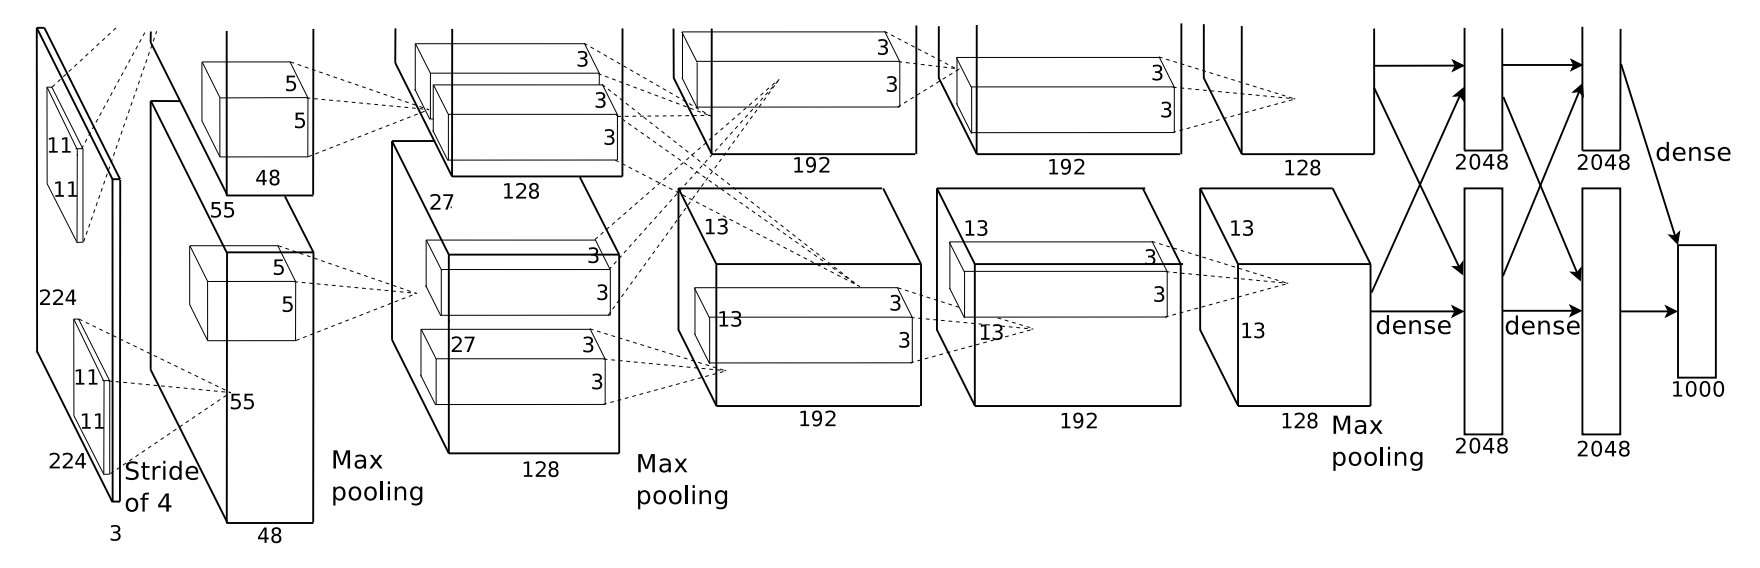
\includegraphics[width=\textwidth]{endoscopy_resources/alexnet.png}
    \caption{Architecture of AlexNet.  \cite{AlexNet}}
    \label{fig:alexnet_arch}
\end{figure}

\subsection{GoogLeNet / Inception} 
The GoogLeNet \cite{inception} was introduced in 2014, it consists of 22 layers together with the Inception Module which described in Figure \ref{fig:inception_block}. Inspired by the fact that salient parts inside an image can have extremely large variation in size and as a result, it is very difficult to choose the right convolution kernel. Because of this, convolution kernels at multiple scales: $1\times1 conv$, $3\times3 conv$, $5\times5 conv$ are done altogether for the previous input, and stack together again at output. The goal of the $1\times1  conv$ is reducing the dimensions of features space. Different kinds of features are extracted because multiple scale of convolutions as well as max pooling are tried simultaneously. Popular versions of InceptionNet includes: Inception v1 \cite{GoogleLeNet}, Inception v2 and  Inception v3 \cite{InceptionV2}, Inception v4 and Inception-ResNet \cite{InceptionV4}.
\begin{figure}[thb]
    \centering
    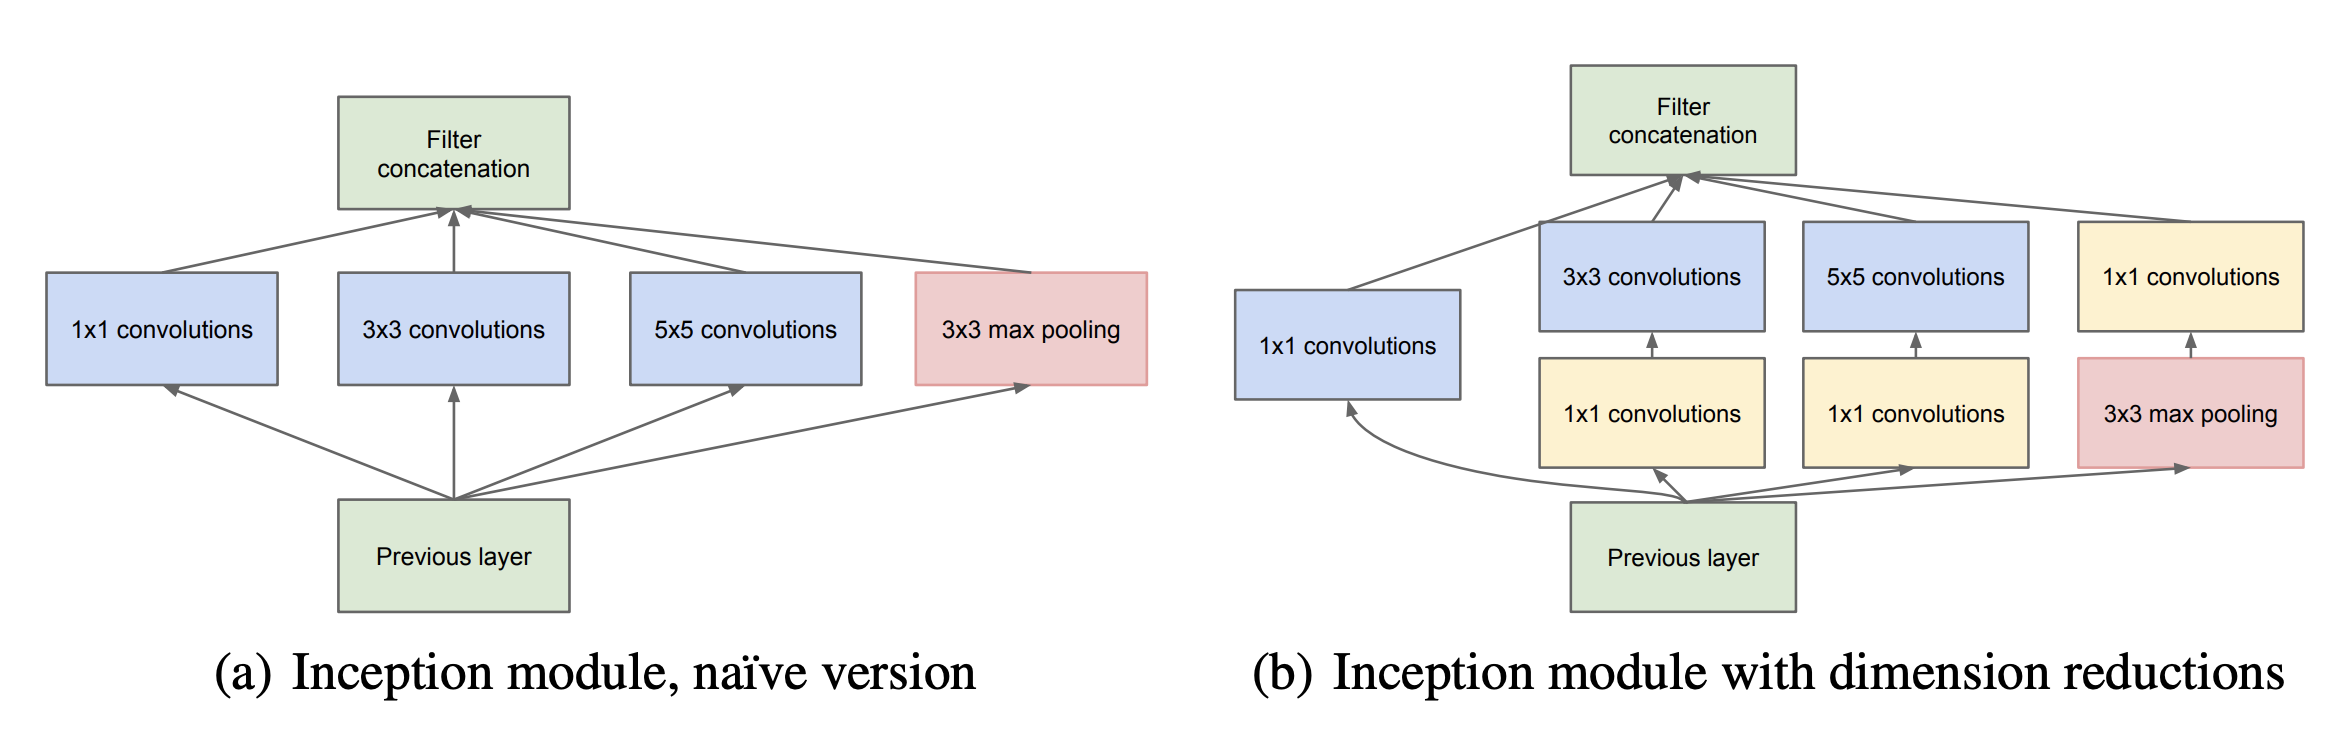
\includegraphics[width=\textwidth]{endoscopy_resources/inceptionnet.png}
    \caption{Inception block. \cite{inception}}
    \label{fig:inception_block}
\end{figure}

\subsection{Residual Neural Network (ResNet)}
In 2015, He et al. introduced the first Residual Neural Network \cite{Resnet} architecture that apply shortcut connections in some layers. Image of a Single Residual Block is given in Figure \ref{fig:single_res}. Different with traditional neural networks where each layer is fed into the next layer consequently, residual blocks can not only feed into the next layer but also into the layers that 2-3 hops away. Thanks to its special design, ResNet allows the flow of memory or information from the initial layers to the last and solving a part of degradation problem that usually happened with deep learning models. ResNet architecture can gain accuracy from considerably increased depth, up to 152 layers. Different architectures of ResNet which are common used in practice are shown in Figure \ref{fig:resnet_arch}.

\begin{figure}[thb]
	\centering 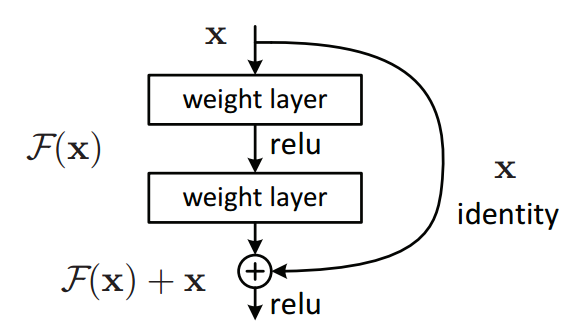
\includegraphics[width=0.5\columnwidth]{endoscopy_resources/single_residual_block.png}
	\caption[Single Residual Block.]{Single Residual Block.\footnotemark.}
	\label{fig:single_res}
\end{figure}
\footnotetext{\url{www.towardsdatascience.com}}

\begin{table}[thb]
    \centering
    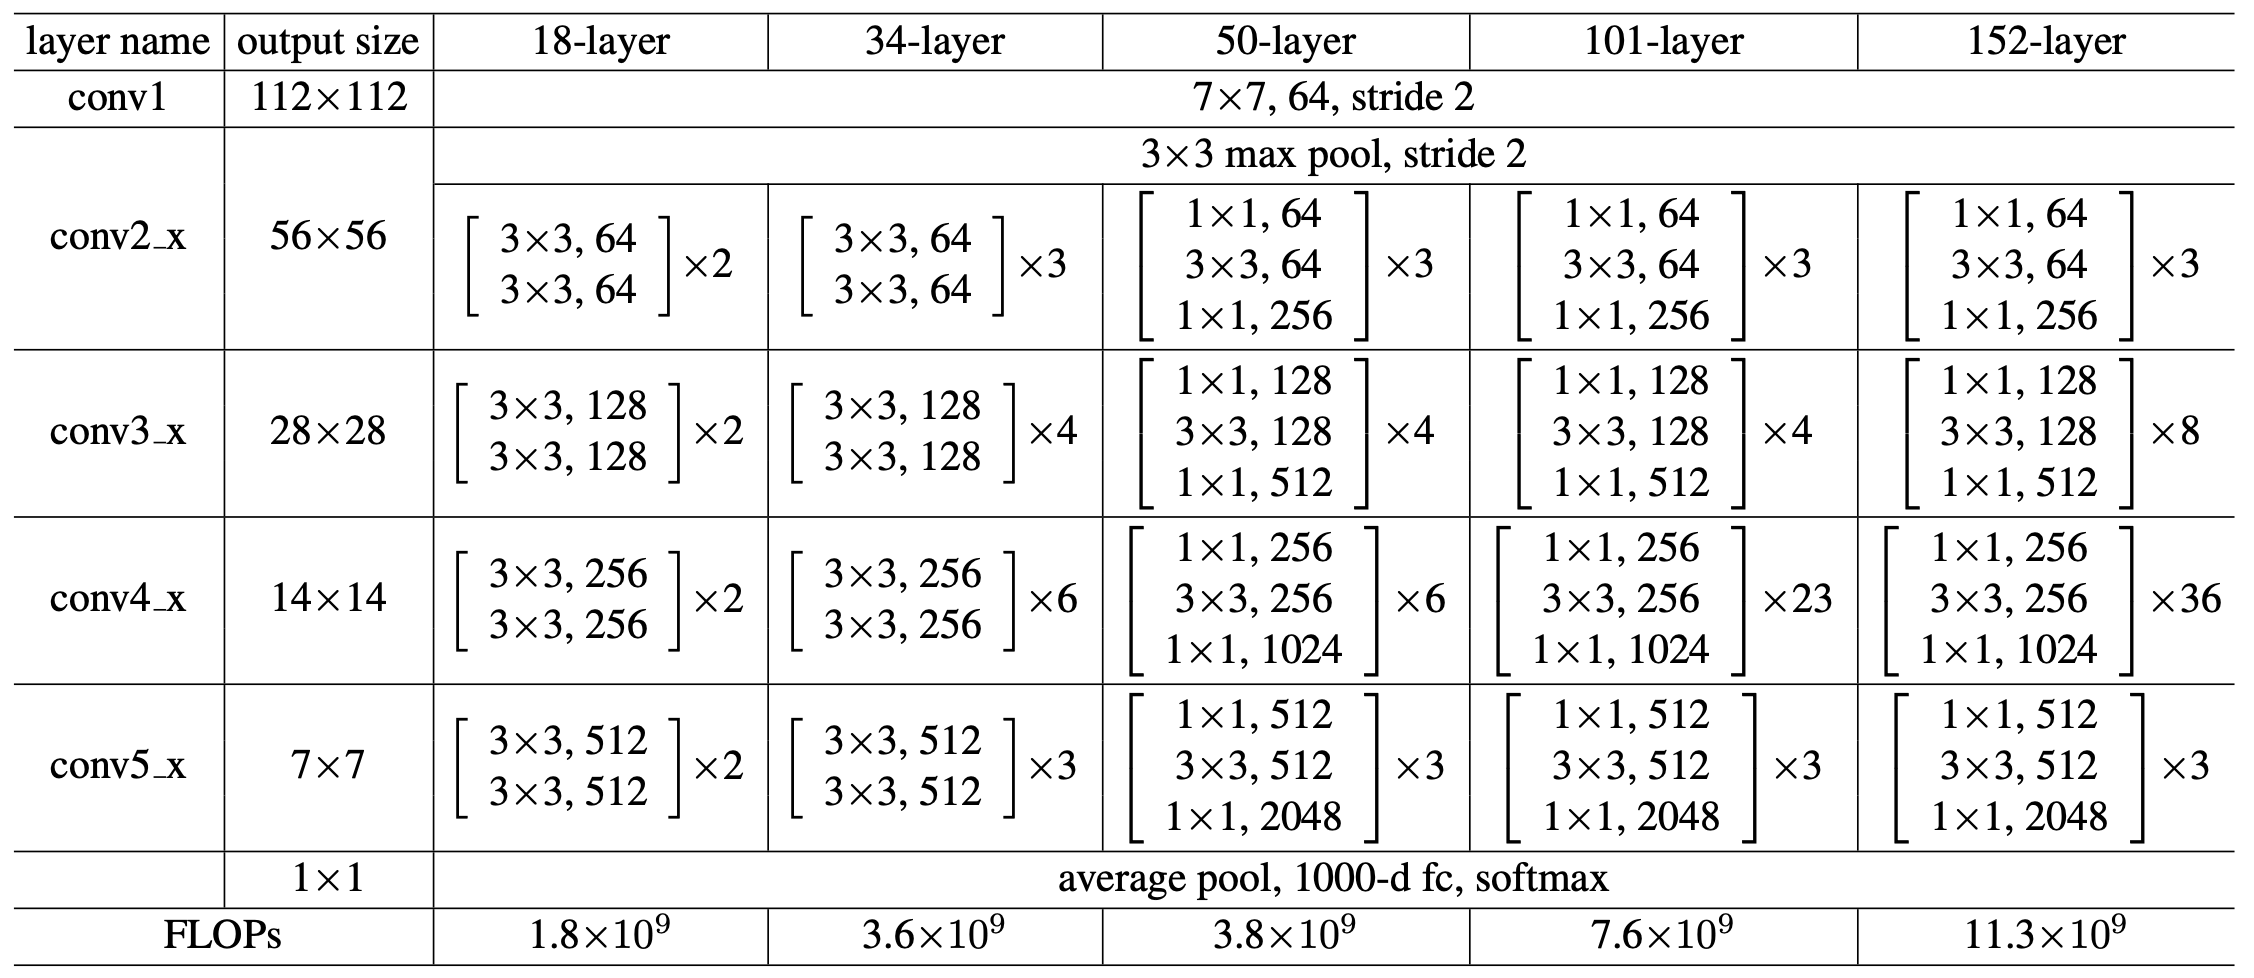
\includegraphics[width=\textwidth]{endoscopy_resources/resnet_archi.png}
    \caption{Different architectures of ResNet. Residual blocks are shown in brackets. \cite{Resnet}}
    \label{fig:resnet_arch}
\end{table}

\subsection{DenseNet}
In other to strengthen features propagation and alleviate the vanishing-gradient, DenseNet \cite{DenseNet} was introduced in 2017 that each layer takes all preceding feature-maps as input and its own feature-maps are used as inputs into all subsequent layers. Figure \ref{fig:dense_net} illustrates a 5-layer dense block with a growth rate of $k = 4$.
\begin{figure}[thb]
    \centering
    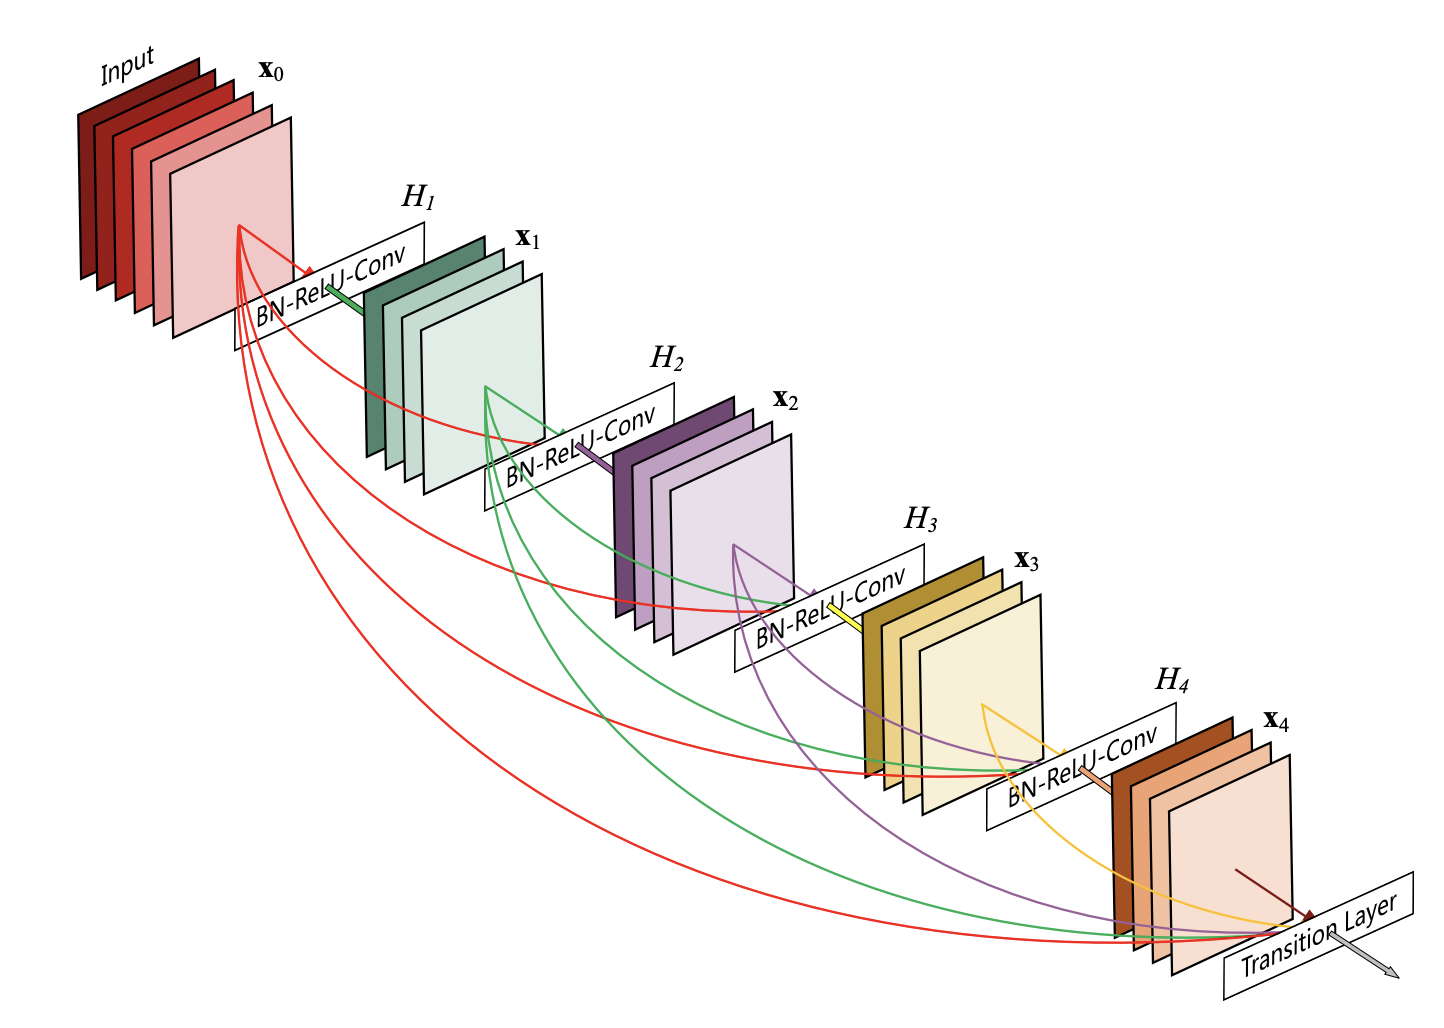
\includegraphics[width=\textwidth]{endoscopy_resources/densenet.png}
    \caption{A 5-layer dense block. \cite{DenseNet}}
    \label{fig:dense_net}
\end{figure}

\section{Object Detection}
Recognizing all objects with a given set of classes is one of the challenge in Computer Vision with a lot of approaches achieving high accuracy, such as Single-Shot Multibox Detector \cite{SSD}, Fast R-CNN \cite{FastRCNN}, Faster R-CNN \cite{FasterRCNN}, YOLO \cite{YOLO}, YOLOv2 \cite{YOLOv2}, YOLOv3 \cite{YOLOv3}. However, in the context of this work, we deiced to investigate and utilize the Faster R-CNN architecture.
\subsection{YOLO}
You Only Look Once (YOLO) \cite{YOLO} is an unified single-scale object detector that allows end-to-end training and real-time speed detection while maintaining high average precision. Introduced in 2016, the idea of YOLO is that a given input image can be divided into an $S \times S$  grid. For each cell in the grid, $B$ bounding boxes, confidence score for each box and $C$ class probabilities are predicted by the model. Figure \ref{fig:yolo_arch} shows the model of YOLO. A number of improvements are conducted on YOLO and put into practice as different versions i.e YOLOv2 \cite{YOLOv2}, YOLOv3 \cite{YOLOv3}.
\begin{figure}[thb]
    \centering
    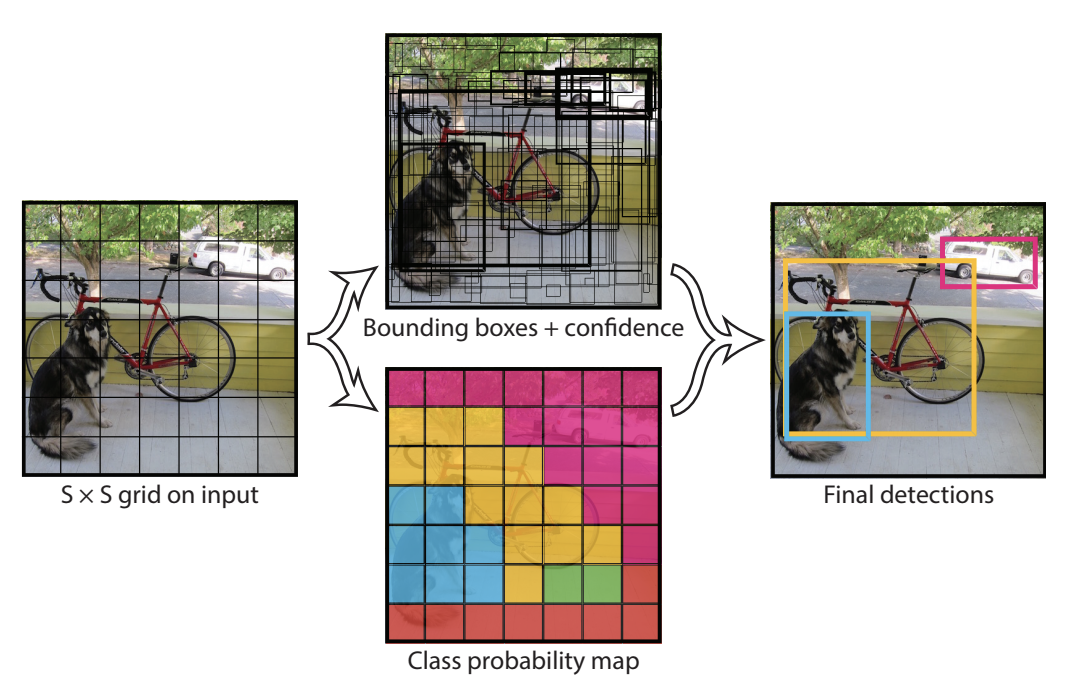
\includegraphics[width=0.7\textwidth]{endoscopy_resources/yolo.png}
    \caption{The model of YOLO \cite{YOLO}.}
    \label{fig:yolo_arch}
\end{figure}

\subsection{Faster R-CNN}
In general, both R-CNN \cite{RCNN} and Fast R-CNN \cite{FastRCNN} share a same approach. Firstly, selective search (SS) \cite{Uijlings2013} is used to generate region proposals. Secondly, a CNN-based network is applied to classify objects and detect the corresponding bounding box in those proposals. However, another approach is conducted on Faster R-CNN \cite{FasterRCNN} which uses a CNN architecture called Regional Proposal Network (RPN) instead of SS. Especially, this CNN is also shared with detection network and the average inference time is then reduced. Thus, the overall network is illustrated in Figure \ref{fig:frcnn_arch}.

\begin{figure}[thb]
    \centering
    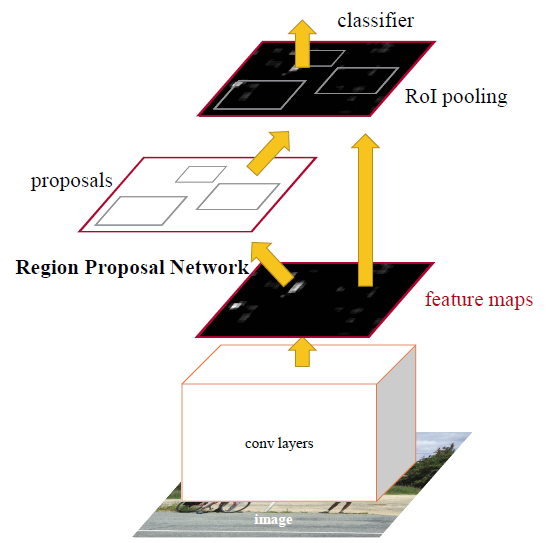
\includegraphics[width=0.7\textwidth]{endoscopy_resources/frcnn_arch.png}
    \caption{Faster R-CNN - a single, unifed network for object detection \cite{FasterRCNN}.}
    \label{fig:frcnn_arch}
\end{figure}

The pipeline of the RPN module of Faster R-CNN architecture is as follow:
\begin{figure}[thb]
    \centering
    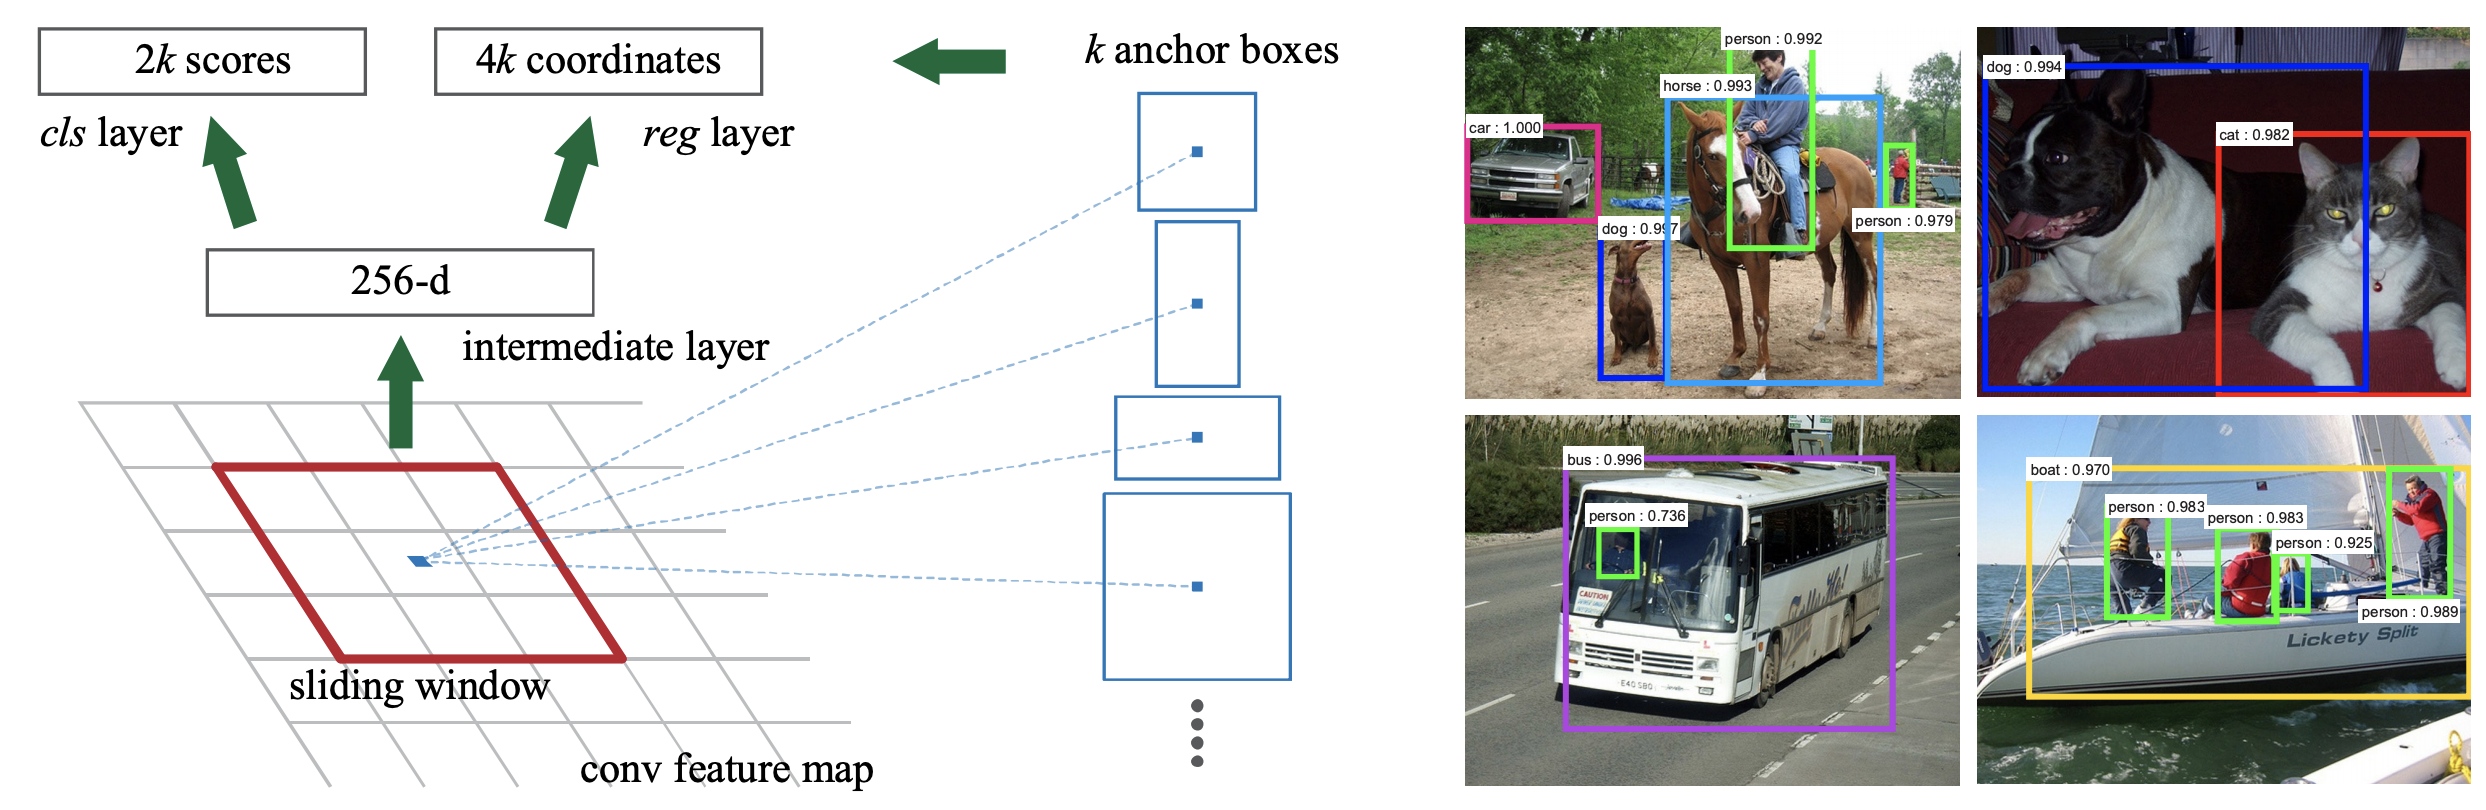
\includegraphics[width=0.9\textwidth]{endoscopy_resources/frcnn_rpn.png}
    \caption{Regional Propasal Network of Faster R-CNN (left) and example detections by using RPN proposals on PASCAL VOC 2007 (right) \cite{FasterRCNN}.}
    \label{fig:frcnn_rpn}
\end{figure}

\begin{itemize}
    \item The input image is inferred through deep convolution layers and features maps of its image are extracted.
    \item In the RPN module which is given in Figure \ref{fig:frcnn_rpn} (left), a sliding window is slidden over the features map. At each position, $k$ anchor boxes which have various scales and aspect ratios are used for generating region proposals.
    \item A $cls$ layer output $2k$ scores implies whether there is object or not for $k$ boxes, respectively.
    \item A $reg$ layer  output $4k$, regarding to the coordinate positions of $k$ boxes.
    \item Finally, all of the outputs are used to adjust the network to learn more accurate, the author defined the following loss function:
    \begin{equation}
        L(\{p_i\}, \{t_i\}) = \dfrac{1}{N_{cls}}\sum_{i} L_{cls}(p_i, p_i^{*}) + \lambda\dfrac{1}{N_{req}}\sum_{i}p_i^{*}L_{reg}(t_i, t_i^{*})
    \end{equation}
    It is noticeable that the above equation is the sum of two smaller loss function. The first part is the loss function for classification and the second part is for the regression. Here, $p_i$ and $t_i$ stand for the output of two layers of RPN, respectively. $p_i^{*}$ and $t_i^{*}$ are the ground-truth labels regarding to whether the given anchor is positive or negative (contains object or not) and the corresponding box is associated with a positive anchor.
\end{itemize}

Except the differences in the RPN module which is described above, the remaining part of Faster R-CNN is similar to the Fast R-CNN \cite{FastRCNN}. Consequently, after performing the ROI Pooling, the pooled area goes through CNN and two Fully Connected branches for class softmax and bounding box regression.

\subsection{RetinaNet}
Different with Faster R-CNN which is a two-stage detector, the RetinaNet  \cite{Retina} is a one-stage network architecture uses a Feature Pyramid Network (FPN) \cite{FPN} backbone on top of a feed forward ResNet architecture. The performance of both YOLO and Faster R-CNN mention above relies on choosing the right anchor size for each training dataset. Outcomes of RetinaNet compared to them is that it is possible to solve the multi-scale problems and generate a rich, multi-scale convolutional feature pyramid which can be further fed to sub-networks like classifying anchor boxes regressing anchor boxes to ground-truth object boxes. Despite having a simple design, the network proved to be surpassing all existing state-of-the-art two-stage detectors and still have a fewer inference time. The RetinaNet architecture is illustrated in Figure \ref{fig:retina_arch}.

\begin{figure}[thb]
    \centering
    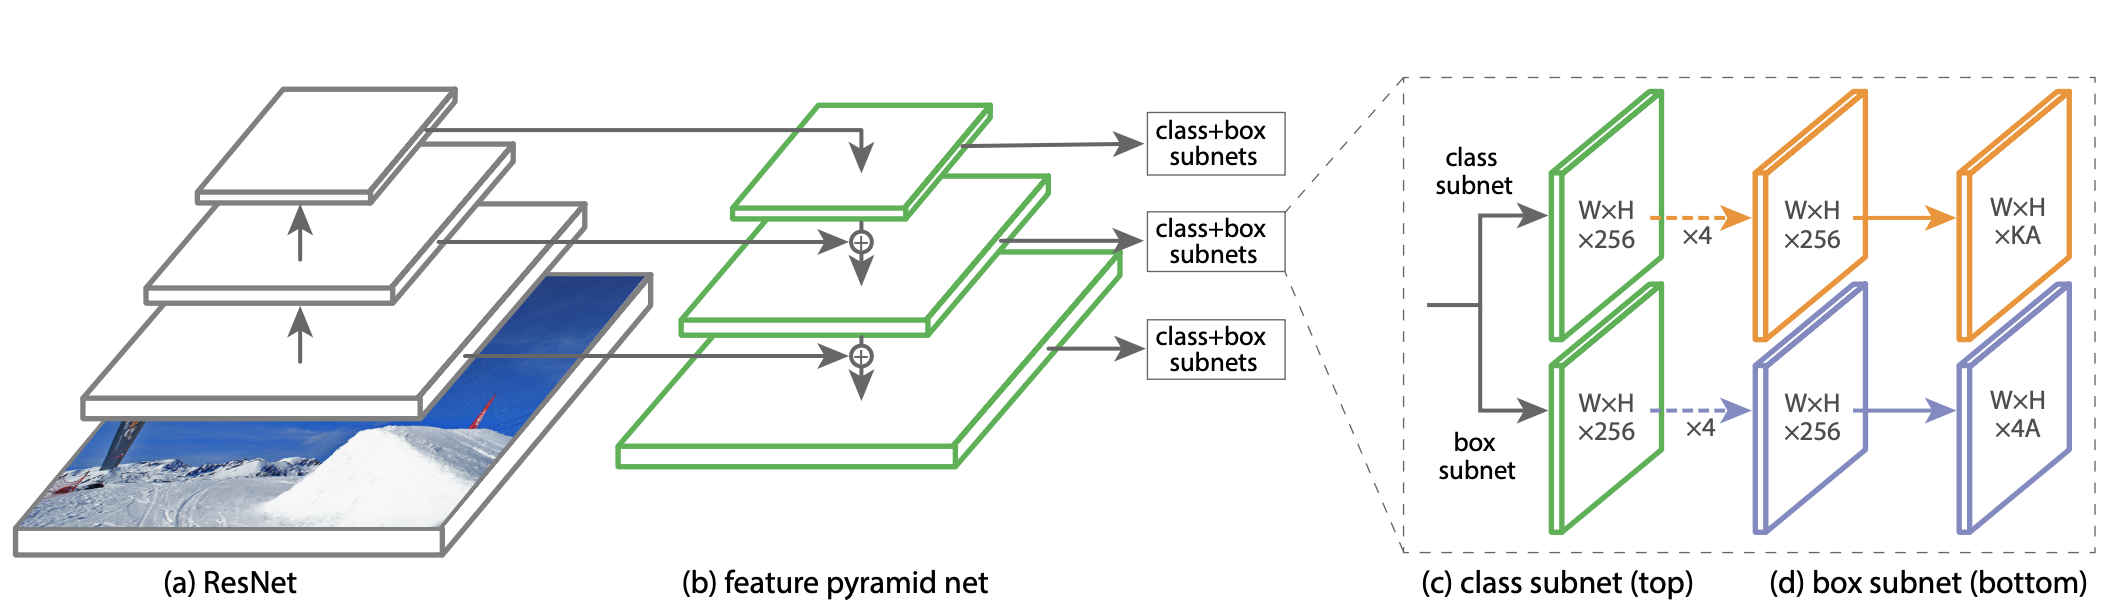
\includegraphics[width=\textwidth]{endoscopy_resources/retinanet.png}
    \caption{The RetinaNet architecture.\cite{Retina}}
    \label{fig:retina_arch}
\end{figure}
\section{Multimedia Assisted Diagnosis Systems}
The detection of abnormalities and diseases in early stages can significantly improve the chance of successful treatment and survival for patients. Multimedia community together with computer scientists can help medical doctors to improve the healthcare system through the application of their knowledge and methods to reach the next level of computer and multimedia assisted diagnosis. In details, these applications can solve a number of difficulties in processing images taking from medical devices. There is a need for an automatic assisted diagnosis system that can process, analysis, and retrieval on medical image and video. The key of these system is how to extract and integrate medical knowledge of experts on analyzing information from medical sensors with high accuracy and require as less as training data as possible. An example of such system is the EIR that conducted during the work of Michael et al. \cite{teammates} and illustrated in Figure \ref{fig:eir_system}. This system supports endoscopists in  the
detection and interpretation of diseases in the entire GI tract.
\begin{figure}[thb]
    \centering
    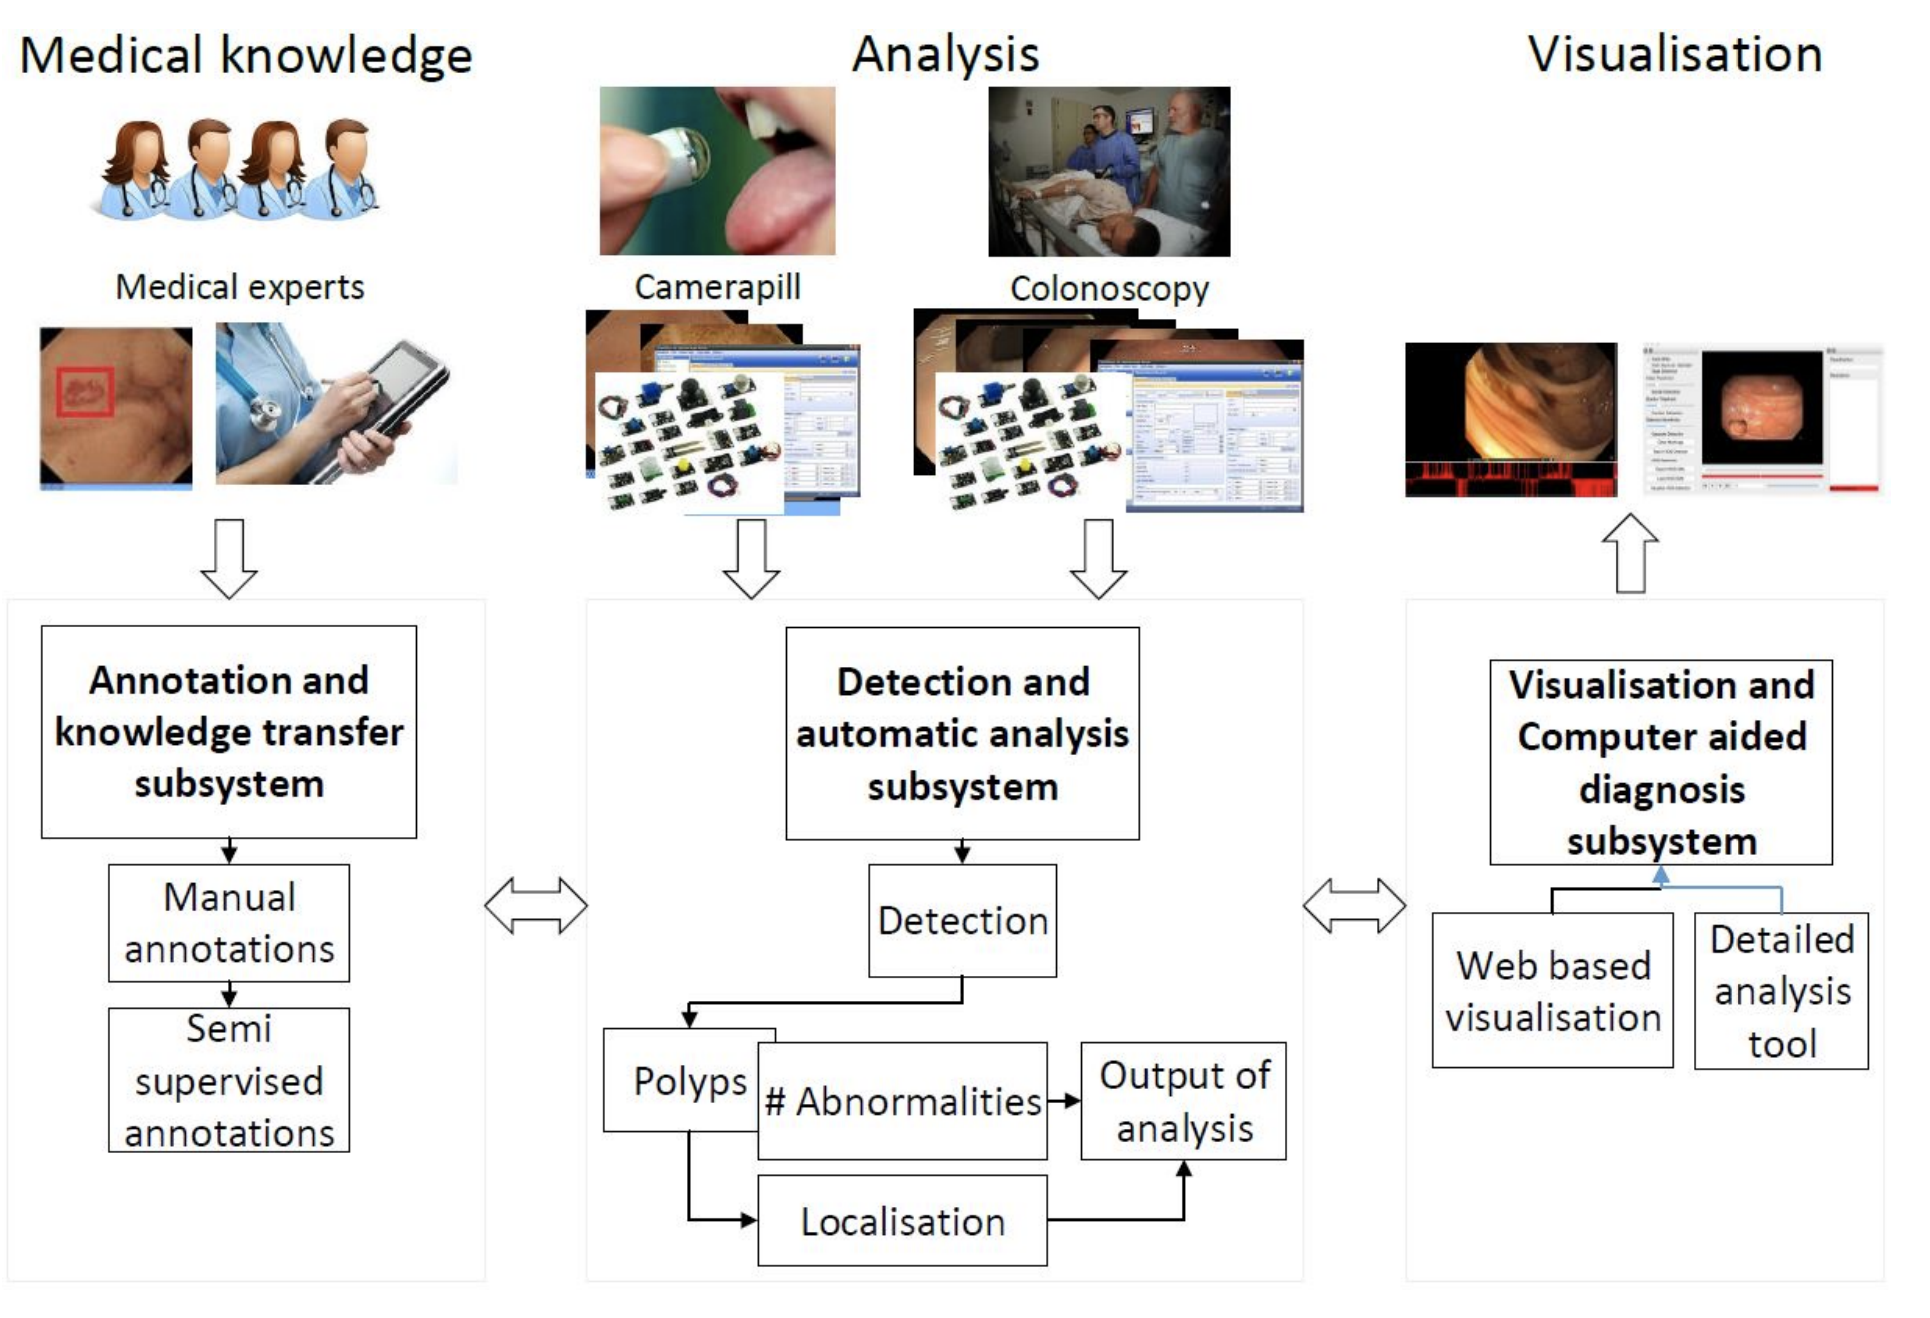
\includegraphics[width=0.9\textwidth]{endoscopy_resources/eir_system.png}
    \caption{EIR system: annotation and knowledge transfer, detection and automatic analysis and computer aided diagnosis.}
    \label{fig:eir_system}
\end{figure}

Beside  endoscopy examination, there are various field in medical diagnosis that can benefit. Most of the works conducted took the newest achievements of Convolutional Neural Network (CNNs). In Cardiac, Chest and Abdominal diagnosis, Tanno et al. \cite{Tanno} proposes a real time classification for vein compressibility analysis from Ultrasound signal. In order to build a system that can classify skin lesion automatically, Zhang et al. \cite{Zhang} has successfully introduced a system that apply deep learning model to overcome intra-class variation and inter-class similarity of skin lesions. Meanwhile, ultrasound images have been successfully classified and tumor malignancy can be detected automatically with CNNs network by the work of Liu et al. \cite{10.1007/978-3-030-00934-2_96}. Nevertheless, the results of this research showed that CNN classifier can not only perform a reasonable performance in predicting breast cancer, but also localize potential lesion regions which can be integrated into the breast ultrasound system in the future.

% Tackling the challenge can for example be addressed by leveraging techniques from multiple multimedia-related disciplines, including methods such as machine learning (classification), multimedia content analysis and multimodal fusion.

\section{Approaches in Endoscopic Images Analysis}
\subsection{Color space and handcrafted features approaches}
Early approaches that tackle with endoscopic image analysis usually work on the bleeding detection problem. Obviously, a bloody region usually has salient color which is significant different from other background areas. A simple approach is using color threshold and applying some handcrafted features in order to localize bleeding symptoms. Shah et al.\cite{HSIColorDomain} and Jung et al.\cite{active_blood_detect} proposed several solutions using color domain and region segmentation. Meanwhile, Novozamsky et al. \cite{blood_detection_color} proposed two technique in counting the number of pixels and localization of bloody region. The first one is defining color spaces that provides good separability of blood pixels. The second is based on an assumption about the shape and size of blood spot and use edge detectors.
Intermediate steps of the second technique are given  
in Figure \ref{fig:blood_detect_color}.

\begin{figure}[thb]
    \centering
    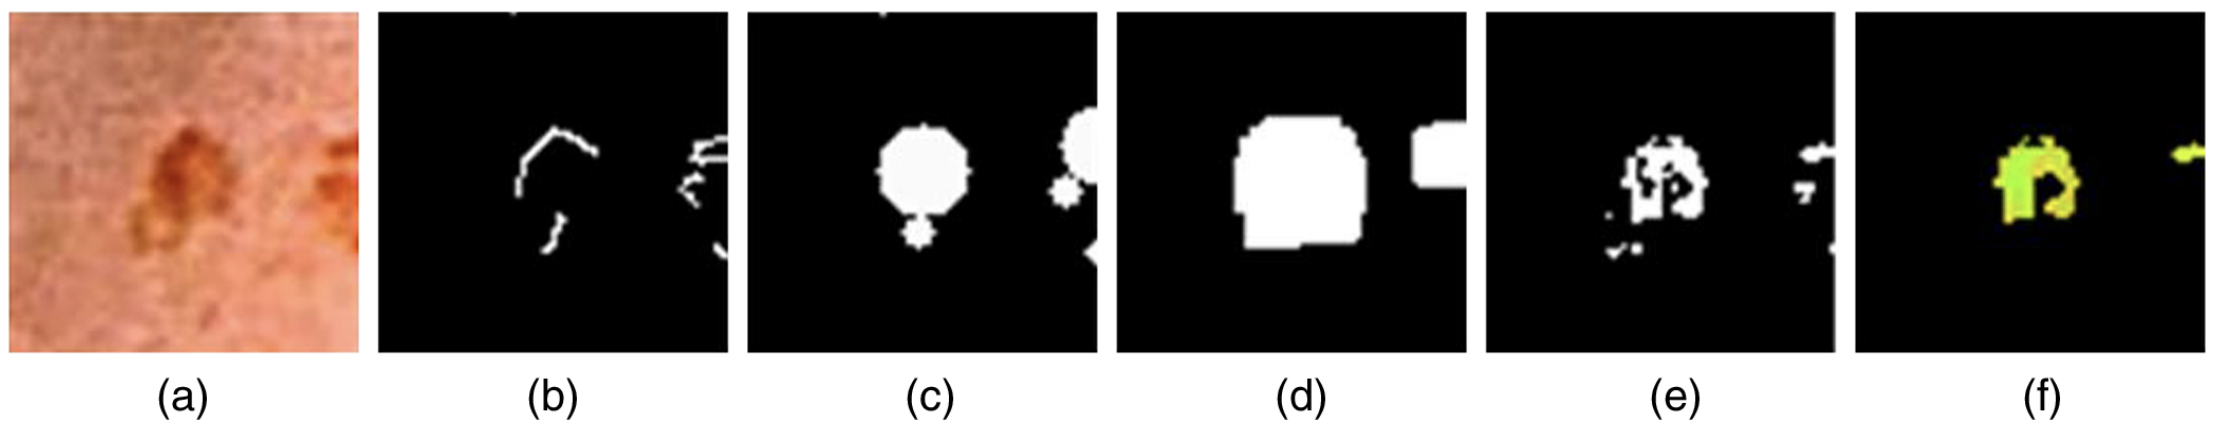
\includegraphics[width=\textwidth]{endoscopy_resources/blood_color.png}
    \caption{Blood detection with the second method.  (a) Input image. (b) Output of Canny detector. (c) Approximate closed-boundary regions. (d) Morphological operation. (e) At the same time, the input image (a) is converted to HSV and potential blood pixels are masked. (f) The output created by intersection of (d) and (e).\cite{blood_detection_color}}
    \label{fig:blood_detect_color}
\end{figure}


\subsection{Machine learning approaches}
Iakovidis et al. \cite{bloodsalientsuperpixels} proposed a solution to detect blood inside endoscopic images which based on a definition of superpixel saliency. Using the information about their color, the
saliency of superpixels is assessed and
enabling the identification of image regions that are likely to contain blood. The blood patterns are recognized by their color features using a supervised learning machine. Proposed solution is illustrated in Figure \ref{fig:super_pixel} through the visualizations of each step.
\begin{figure}[thb]
    \centering
    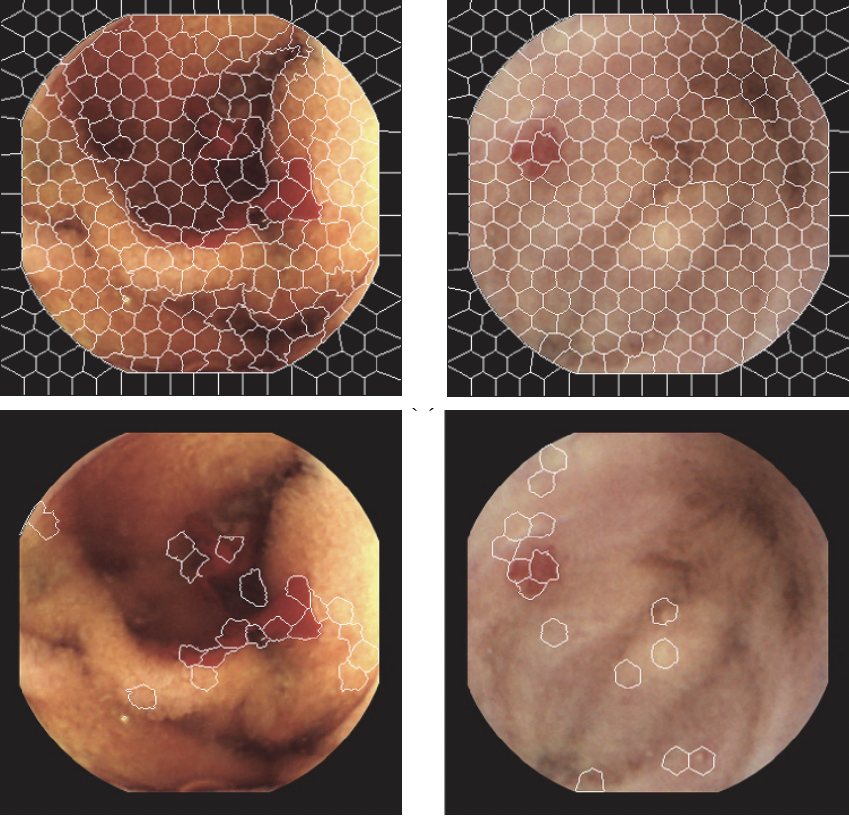
\includegraphics[width=0.6\textwidth]{endoscopy_resources/super_pixels_salient.png}
    \caption{Endoscopic blood detection based on Salient Super pixels.\cite{bloodsalientsuperpixels}}
    \label{fig:super_pixel}
\end{figure}
\subsection{Deep-learning approaches}
In the field of medical image processing, deep neural networks has proved it advantages in order to solve several problems related to endoscopic images of the human gastrointestinal (GI) tract. Particularly, to localize and identify polyps within real-time constraint, deep CNNs has recently shown an impressive potential when achieving up to 96.4\% accuracy - published in 2018 by Urban G et al. \cite{urban_tripathi_alkayali_mittal_jalali_karnes_baldi_2018}. Another interesting article of Satoki Shichijo et al. \cite{Shichijo2017} also applies multiple deep CNNs to diagnose Helicobacter pylori gastritis based on endoscopic images. According to the research, after training with more than 30,000 endoscopic images, the accuracy of the CNNs is comparable to that of endoscopists. CNNs approaches is substantially shorter time and contribute to reducing the efforts of endoscopists. Further, gastrointestinal bleeding detection using deep CNNs on endoscopic images has been successfully done and published by Xiao Jia et al. \cite{jia_meng_2016} with impressive $F_1$ score up to 99.55\%. The CNNs architecture conducted in this research is shown in Figure \ref{fig:cnns_bleeding}.

\begin{figure}[thb]
    \centering
    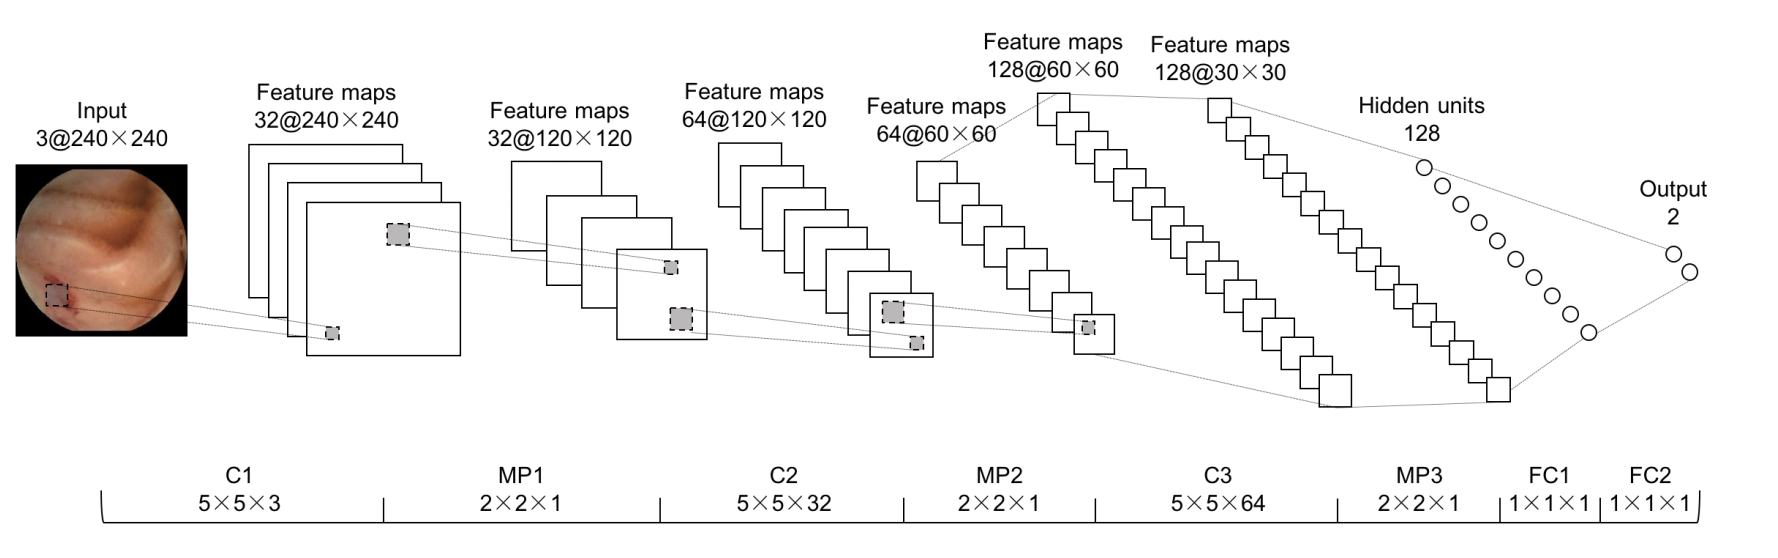
\includegraphics[width=\textwidth]{endoscopy_resources/cnns_bleeding_detection.png}
    \caption{Gastrointestinal bleeding detection CNNs architecture proposed by Xiao Jia et al.  \cite{jia_meng_2016}}
    \label{fig:cnns_bleeding}
\end{figure}

% \section{Dataset Augmentation}
% One of the biggest problem of Deep Neural Network is that it requires a large number of training samples. However, in some cases it is insufficient to have such amount of data. Applying several simple augmentation strategy like Random Flip, Random Rotation, Random Brightness and Contrast augmentation can also be applied. Novel approaches in data augmentation are taking into account where Another approach like using \cite{DBLP:journals/corr/KhorevaBIBS17}

\section{Image Segmentation}

Beside the object detection problem, image segmentation requires not only detected and classified bounding boxes around the interested objects but also the accurate contours of those ones. These results from image segmentation provide finer features about the segmented objects, such as size, shapes, orientation, etc, that can further be used to analyze the object's properties. There are two main degrees of solving this kind of problem: semantic segmentation and instance segmentation. The former are focusing on grouping the pixels in image into a semantically meaningful results, i.e. object category, while the latter requires a further instance separation step to make each instance in same object category distinctively. Figure \ref{fig:3_object_vs_instance} visualizes the desired results of each type of problems, including semantic segmentation and instance segmentation.

\begin{figure}[thb]
    \centering
    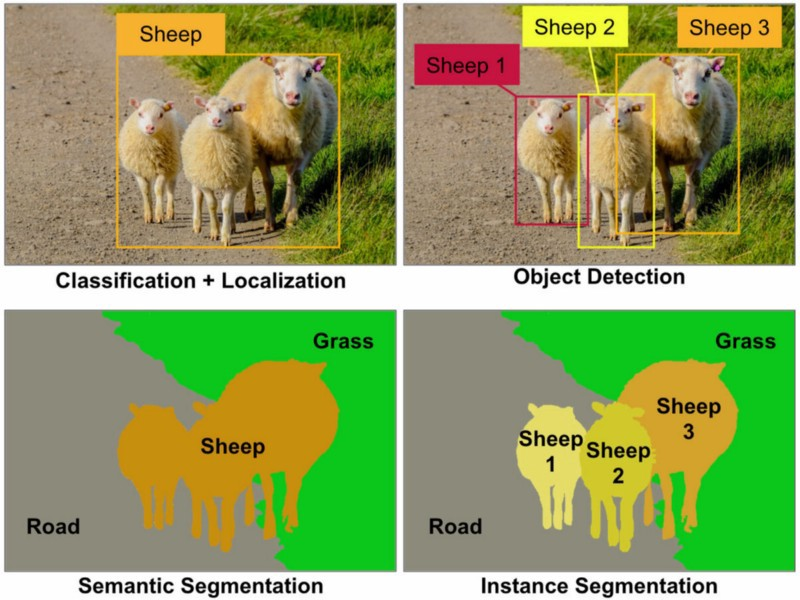
\includegraphics[width=\textwidth]{resources/3_object_vs_instance.jpeg}
    \caption{Difference between desired results from different tasks in Computer Vision \cite{instace_vs_object}.}
    \label{fig:3_object_vs_instance}
\end{figure}

Well-known approaches before deep learning often exploit the relationship of color, intensity or texture of region around the interested pixel. K-means clustering \cite{kmean} or other graph-based algorithms such as minimum spanning tree based segmentation (MST based segmentation), energy minimization using Graph Cuts \cite{FastGraphCuts, EfficientGraphBasedSegmentation}, GrabCut \cite{GrabCut}, etc. are often utilized to do region-based segmentation. However, some variations in the data, such as color, illumination, texture or non-rigid orientation, makes these approach difficult to generalize well in real-life conditions. 

Inheriting from recent achievement of deep learning in solving object detection problems, new neural network achitecture has been proposed to tackle the segmentation problems, in both semantic level and instance level. PASCAL VOC \cite{PASCALVOCDataset} and MSCOCO \cite{MSCOCODataset} become standardized datasets for the segmentation problems. Many recent proposed methods try to beat the state-of-the-art on these datasets, however, most of them share a basic underlying designed architecture which is known as Fully Convolutional Networks (FCNs) \cite{FCNs}. This is a typical networks for semantic segmentation by replacing the last fully connected layers of object detection network by a decoder network which restores the original resolution of input image by using transposed convolutional layers which are may known as deconvolutional layers. In more details, the network must consist of two main stages: Encoder stage which converts image in original pixel space to a learned feature space and Decoder stage which maps the extracted features to the result space, which often has same dimension as the original input image. An example of this process is illustrated in Figure \ref{fig:CL_DL}. DeepLab \cite{DeepLabv1,DeepLabv2,DeepLabv3,DeepLabv3+}, Pyramid Scene Parsing Net \cite{PSPNet} for semantic segmentation or Mask R-CNN \cite{MaskRCNN} and MaskLab \cite{MaskLab} for instance segmentation are well-known approaches lately designed based on this architecture.

\begin{figure}[thb]
\centering
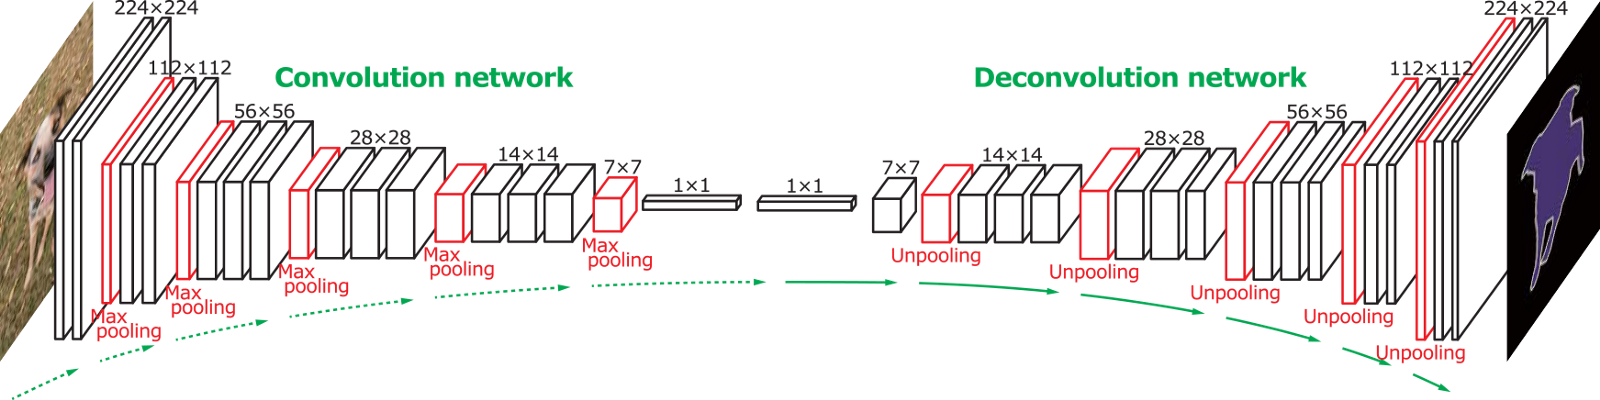
\includegraphics[width=1\textwidth]{resources/3-conv-deconv.png}
\caption{Two stages of FCNs: Encoder process with convolution network and decoder process with deconvolution network \cite{conv_deconv}.}
\label{fig:CL_DL}
\end{figure}

U-Net \cite{unet} shares some similarity in the network design with FCNs \cite{FCNs}; however, the long skip connections are included to connect the features from encoder branch to the decoder branch. The authors argues that the features from encoder stages containing low-level features such as edges, contours, etc. that needs to be preserved during the decoder stages. To achieve this property, features from encoder layers at the same level could be simply copied and concatenated with the deconvolved results, then go through a convolutional layers, yielding a combined features between encoder and decoder branch. These features, as described in the U-Net paper \cite{unet}, contain discriminative property that can help pixels, especially pixels on boundary, to have better classification results. Figure \ref{fig:u_net} visualizes the design of a typical U-Net architecture.

\begin{figure}[thb]
    \centering
    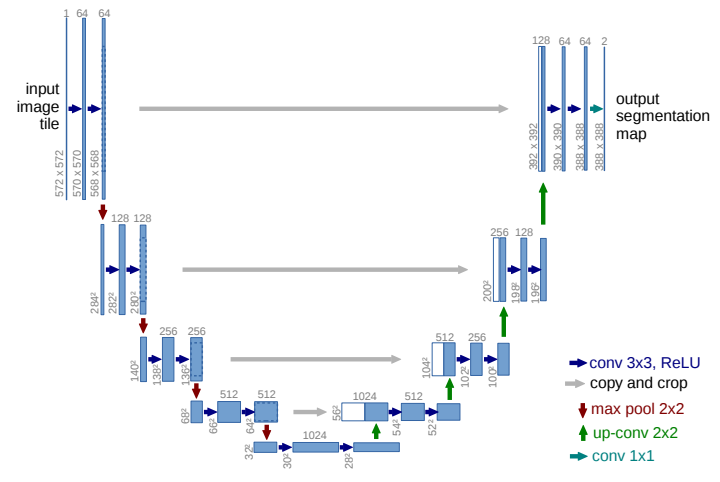
\includegraphics[width=\textwidth]{resources/3_u_net.png}
    \caption{U-Net architecture \cite{unet}.}
    \label{fig:u_net}
\end{figure}

\section{Nuclear segmentation in Medical Image Analysis}

In this section, we review approaches used to solve segmentation problems in medical image analysis. These methods are grouped in each subsections to better describe the merit of each family solution. Most of materials in this section are referenced from these comprehensive reviews \cite{review_seg_overall}, \cite{survey_on_medical_image_analysis}. 

\subsection{Intensity thresholding}
This could be the first and simplest method for nuclear segmentation. Based on the sufficient and consistent distinction of the intensity distributions between nuclei/cells and the background, the Otsu’s method \cite{Otsu} performs statistical discriminant analysis of the image intensity histograms, and chooses an optimal threshold value by maximizing the interclass variance. To deal with the noise or nonuniform illumination, image is divided into sub-images to perform local thresholding. This requires an additional parameter, which is the local region size, needed to tune during developing the algorithm. Some proposed methods use the merit of intensity thresholding to separate the nuclei from background such as Callau \textit{et al.} \cite{Callau2015} for segmenting the epithelial cell areas in breast cancer TMA images, Keenan \textit{et al.} \cite{Keenan2000AnAM} for isolating nuceli in cervical images, etc. 

\begin{figure}[thb]
    \centering
    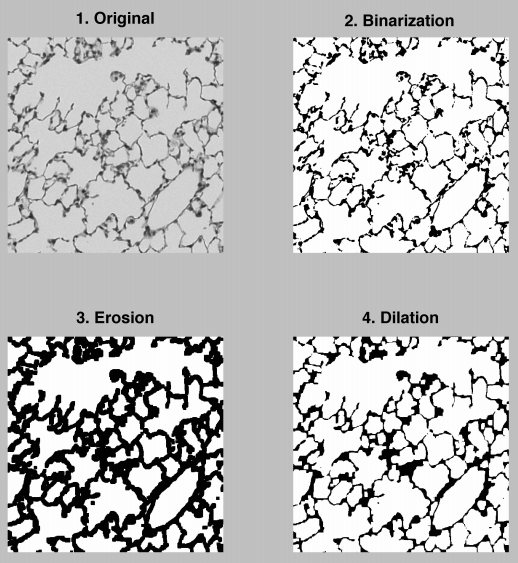
\includegraphics[width=0.5\textwidth]{resources/2_morphological_seg.png}
    \caption{Segmentation of lung patches using binarization, erosion and dilation operators. \cite{morphological_seg}}
    \label{fig:morphological_seg}
\end{figure}

\subsection{Morphology Operations}
By applying thresholding to binarize the input image, erosion and dilation, which are two basic morphology operations \cite{morphology1}, are used to create segmentation results. Iterative erosion operators with increasing scales are applied until obtaining the markers. These markers become cell seeds indicating regions of individual nuclear. Dilation are iteratively used to expand the cell seeds region, creating the final segmentation results. However, for dense cell clumps, this method oftens produce undersegmentation results. Figure \ref{fig:morphological_seg} visualizes the results of each step when morphology operations are applied to do segmentation task on medical images. 

\subsection{Watershed Transform}
In watershed transform \cite{watershed}, an image is viewed as a landscape which the intensity of pixels is considered as altitude. The algorithm starts at the local minima as independent seeds and iteratively adds the connected regions to merge them into nearest union components. In other ways, watershed transform floods the terrain by filling the water from the lowest point in local regions. The dams, which are call watershed lines, are built to prevent water from merging when water from distinct regions is going to meet. The procedure stops when  water reaches the highest point. The main drawback of this approach is that it produces excessive over-segmentation, especially for natural images. There are some works based on this typical idea such as Long \textit{et al.} \cite{long_watershed}, Yang \textit{et al.} \cite{yang_watershed}, etc.

\subsection{Clustering}
K-means clustering \cite{kmean} applied by Kothari et al. \cite{clustering1} to do segmentation in H\&E and IHC stained pathology images or Arif and Rajpoot \cite{clustering2} on nuceli segmentation. Other soft clustering algorithm, such as fuzzy c-mean (FCM) \cite{fuzy}, are also used in nuclei segmentation \cite{parallel_fuzy}. However, due to lack of nucleus shape prior, the cell seed need to be generated to create the number of original groups which lead to unreasonable boundary results. 

\subsection{Graph-based methods}
There are several approaches in the graph-based method to solve nuclear segmentation. Max-flow/min-cut \cite{maxflow} often try to minimize a defined energy function which can separate the nuclei from background. Another approach is normalized cut \cite{normalized_cut} which tries to recursively separate the graph into two disjoint set with a minimum cut. Conditional Random Field (CRF) \cite{crf} is a discriminative graphical model people also often use to do image segmentation. Wu et al. \cite{6157605} applies this idea to do segmentation in cytology images.

\subsection{Deep learning}

With the recent advances of deep learning on other related fields in Computer Vision such as object detection, as well as the increasing amount of training data in medical image analysis, there are a shifting attention of research community from previous mentioned approaches to deep learning. There are a lot of grand challenges in digital pathology, boosting the maturity of this research area. A lot of deep learning methods achieved the highest rank in these challenges, such as Ciresan \textit{et al.} \cite{NIPS2012_4741} in EM segmentation challenge 2012, Xu \textit{et al.} \cite{DBLP:journals/corr/XuLLWLC16} in GLAS for gland segmentation, etc. Ehteshami Bejnordi \textit{et al.} \cite{7243333} even outperform the performance of a pathologist on the test set of CAMELYON16 challenge for processing breast cancer tissue samples. The staining and imaging modality are also diverse, including hematoxylin and eosin staining (H\&E), tumor-infiltrating lymphocytes (TIL), electron microscopy (EM), fluorescent (FL), etc. This demonstrates a great potential of deep learning applied in medical image analysis, especially nuclear segmentation.

\begin{figure}[thb]
    \centering
    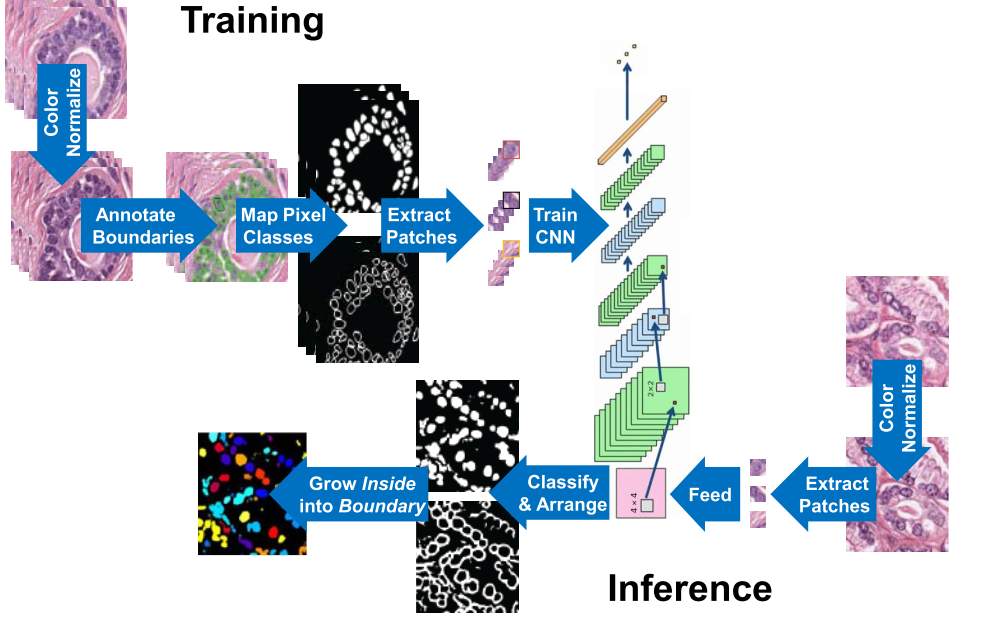
\includegraphics[width=\textwidth]{resources/3-cnn3.png}
    \caption{The proposed pipeline in CNN3 \cite{he_dataset_kumar} to do nuclear segmentation on H\&E stained histopathology images.}
    \label{fig:cnn3}
\end{figure}

One recent remarkable study by Kumar \textit{et al.} \cite{he_dataset_kumar} to perform nuclear segmentation on H\&E stained histopathology images attracts a lot of attention from research community. One of their main contribution is creating a new dataset containing 30 well-annotated images from TCGA project \cite{tcga}. As mentioned in \cite{he_dataset_kumar}, the data comes from 18 different hospitals, covers seven different organs including breast, liver, kidney, prostate, bladder, colon and stomach, both benign and diseased samples. This creates a benchmark for research community to develop nuclear segmentation techniques specially on H\&E stained histopathology images with diverse nuclear types. Besides the proposed dataset, authors in \cite{he_dataset_kumar} also designed an approach to solve the segmentation problems. For better separation touching nuclear, 3-class probability assignment by deep neural network, including inside, outside and boundary, has been proposed. This becomes one of the basic configuration followed by later algorithms. Figure \ref{fig:cnn3} visualizes the pipeline proposed in \cite{he_dataset_kumar} in more details. As the reported result, this approach \cite{he_dataset_kumar} improves the F1-score to about 83\% compared to 40\% of a configuration of Fiji's \cite{fiji} segmentation algorithm. 

\section{Group equivariance in neural network}

\subsection{Equivariant property}

\begin{figure}[thb]
    \centering
    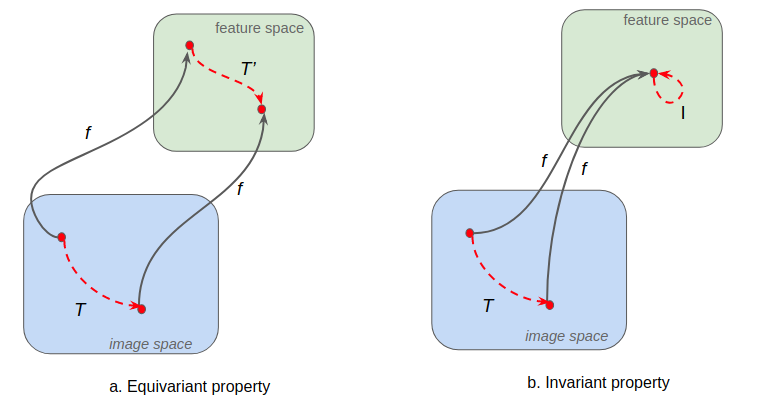
\includegraphics[width=\textwidth]{resources/2_equi_invar.png}
    \caption{Visualization of equivariance and invariance definition.}
    \label{fig:equi_and_invar}
\end{figure}


Let $f(x)$ is a representation of an input image x in the image space. This representation is equivariant to a family of transformations $I$ on image spaces if for any transformation $T \in I$, there exists a corresponding transformation $T'$ on feature spaces, such that

\begin{equation}
    f(Tx) = T'f(x)
\end{equation}

for any input images x \cite{dren}. It means that the representation of transformed input images are predictable if the transformation obeys the  equivariant rule. In case $T'$ equals to identity transformation, the representation remain unchanged no matter the transformed images as versions of input needed to be represented. This property is call invariant. A good classifier should owe this property to produce strong results under the dramatic change in the input space. Figure \ref{fig:equi_and_invar} visualizes the merit of each property including equivarance and invariance in an image space and its corresponding feature space. As proven in \cite{gcnn}, the convolutional neural networks are effective because of weight sharing mechanism, which activates the translation equivariance or translation invariance in most perception task. It means that the feature of shifted version of image feeded to the network is same as the shifted feature of the original images plugged to the same network. However, the features extracted from vanilla neural network cannot be equivariant to other group of transformation such as rotation, reflection, etc. It could be beneficial if these transformations could be cooperated to the network in the equivariant manners. For example, there is a family of special rotation transformations $R = \{R_{\theta} | \theta = k\pi/2, k \in Z \}$ that owns this equivariant property in the mathematics way. Encoding these group equivariance to the network yields the better generalization of the results produced by these architectures.


\subsection{Approaches}
Data augmentation is one way to force the network to learn equivariant/invariant feature representation. During the training process, some transformations could be applied on the input data to expand the input space the network has looked through. With enough capacity and huge amount of training data with defined set of transformations, the network could be able to force this property in its feature representation. However, the input space are often too huge to cover during the training process, there is no guarantee that the network could generalize the equivariant/invariant property outside the training set. Moreover, to learn this property, each parts of the network has to learn different representations of input data, for example different versions of rotation of input image. This sacrifies a lot of network capacity to learn these representation, which could be the duplicate of each others, instead of other useful features. Cooperating the equivariance/invariance to group of transformations could help the network generalizing better in the real-life scenarios.

Test time augmentation is often used to produce the results that are equivariant/invariant to transformations on the input data. For example, to obtain the equivariance/invariance property on the results created by CNNs, the multiple versions of input image are generated by a set of transformations. These images are then used to produce the predictions. The final result is the average ones of multiple transformed versions. This do not require to change any layers in the architecture design; however, it consumes a lot of computation resources to produce one output. Once again, this method does not solve the problem from the original source.  

\begin{figure}[thb]
    \centering
    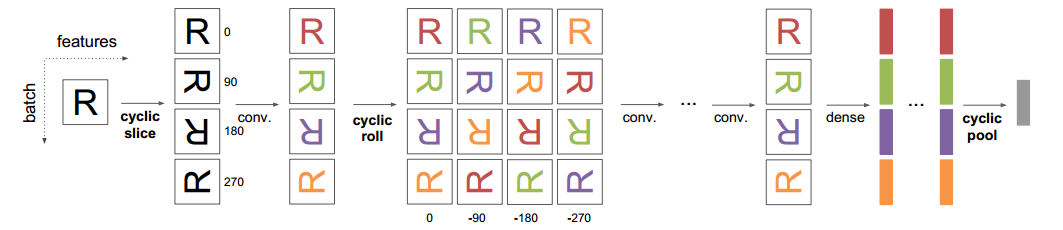
\includegraphics[width=\textwidth]{resources/2_exploting_symmetry.png}
    \caption{The design proposed by Dieleman \textit{et al.} \cite{cyclic_symmetry} to exploiting cyclic symmetry in convolutional neural networks. }
    \label{fig:cyclic_symmetry}
\end{figure}

To exploit cyclic symmetry in convolutional neural networks, Dieleman \textit{et al.} \cite{cyclic_symmetry} introduces four operations that could be used as layers in the design neural network models, enabling partially equivariant to rotations. Cyclic slicing operation produces different rotated versions of input data and stack them into a single batch of training data, while cyclic pooling operation combines different predictions from different rotated copies of input data, merging the batch data created by cyclic slicing operation into a unified one. These two operations focus on converting the space between the input and output while maintaining the equivariance, for example slicing converting the input space to feature space. Cyclic rolling is specially designed to preserved the equivariance in the feature space, which creates the dictionary of all of different rotated versions of extracted features. These features are stacked by cyclic stacking in a mathematics way to preserve the equivariant features. Figure \ref{fig:cyclic_symmetry} visualizes their pipelines to incorporate this property to the network design. Despite the generalization for 90-degree rotation, the extracted features are also partially shown the equivariance to other degrees, which indicates the effectiveness of this design. 

\begin{figure}[thb]
    \centering
    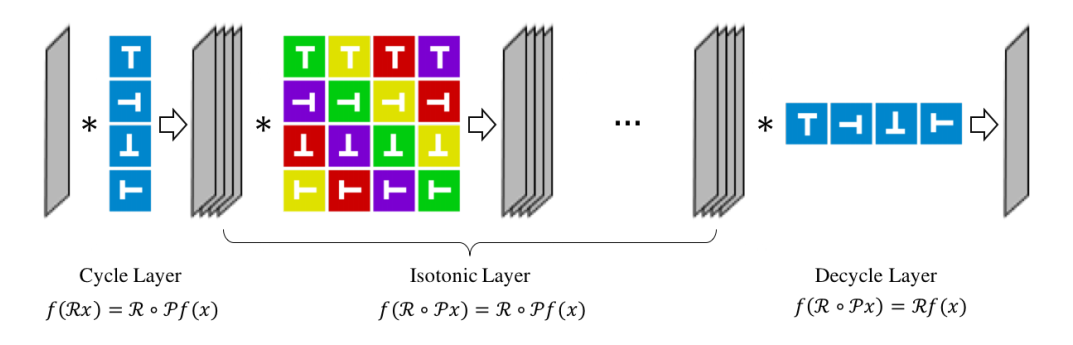
\includegraphics[width=\textwidth]{resources/2_dren.png}
    \caption{The enhancements in the implementation proposed by Li et al. \cite{dren}. Instead of rotating on the feature maps as \cite{cyclic_symmetry}, this method rotates the filters of neural network, saving a lot of memory consumption in the training and inference time.}
    \label{fig:dren}
\end{figure}

Rotating features in the feature space does not require to design any new special layers apart from the current design of vanilla convolutional neural networks. However it consumes a lot of memory because storage of different rotated features. Seeing this pain point, Li et al. \cite{dren} proposed a new approach to implement this idea. Instead of rotating features, they rotate the weights of neural network and use equivalent transformations to create final prediction. All of the proposed layers share the merit with the design from \cite{cyclic_symmetry}. The filters are much smaller than the features, which decrease a huge amount of memory consumption. Figure \ref{fig:dren} visualizes their enhancements in the implementation ideas which are applied on the filters of the neural network, instead of on the feature maps as in figure \ref{fig:cyclic_symmetry}.

Two previous approaches aim to cooperate 90-degree rotation equivariance to the neural network. Marcos \textit{et al.} proposed RotEqNet \cite{DBLP:journals/corr/GonzalezVKT16} to increase the number of rotation degrees that network could produce the equivariant features. Despite freeing the network from learning different features of set of transformed input data, both of two mentioned methods require to store different rotation of features or filters, which partially increases the model size as well as the runtime memory usage. Instead of storing all of the combination of rotated features, RotEqNet \cite{DBLP:journals/corr/GonzalezVKT16} uses the 2D vector filed, which captures the magnitude and orientation of the maximum value across the feature maps. Figure \ref{fig:vector_field} describes their ideas in more detail. Basing on the group theory, Cohen and Welling create a mathematics framework \cite{gcnn} to generalize the equivariance requirement to set of transformations. This does not limit the network on the type of transformations that could be cooperate to its feature representation. For example, the group \textit{p4m} includes the composition of translations, mirror reflections and rotations by 90 degrees about any center of rotation in the grid \cite{gcnn}. The details of this method are discussed in chapter \ref{chap-method}. 

\begin{figure}[thb]
    \centering
    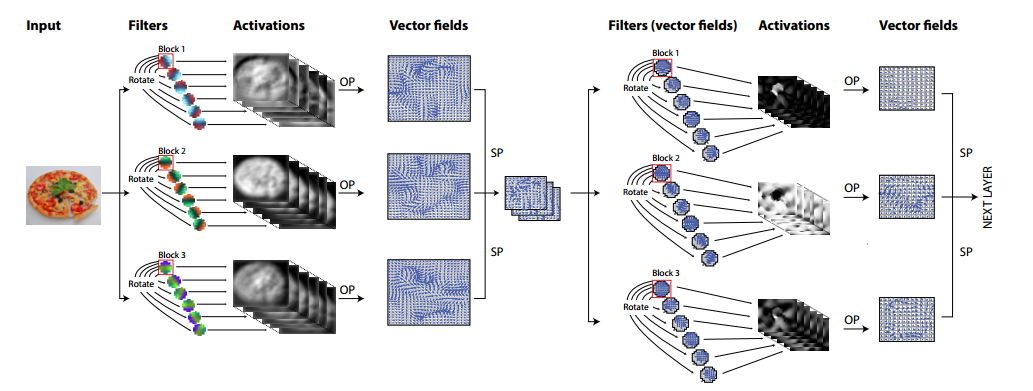
\includegraphics[width=\textwidth]{resources/2_vector_field.png}
    \caption{The RotEqNet proposed by Marcos \textit{et al.} \cite{DBLP:journals/corr/GonzalezVKT16}. This network aims to compact the model in terms of the number of trainable parameters while increasing the amount of number equivariant rotation degrees.}
    \label{fig:vector_field}
\end{figure}

\begin{ChapAbstract}
In this chapter, we give an overview of some works on image classification, object detection, semantic segmentation and instance segmentation. The approach in abnormal findings and anatomy landmark detection in endoscopic image analysis together with nuclear segmentation are discussed in more details. Moreover, we also present the equivariance definition as well as its application in deep neural networks.
\end{ChapAbstract}